% Options for packages loaded elsewhere
\PassOptionsToPackage{unicode}{hyperref}
\PassOptionsToPackage{hyphens}{url}
%
\documentclass[
]{article}
\usepackage{lmodern}
\usepackage{amssymb,amsmath}
\usepackage{ifxetex,ifluatex}
\ifnum 0\ifxetex 1\fi\ifluatex 1\fi=0 % if pdftex
  \usepackage[T1]{fontenc}
  \usepackage[utf8]{inputenc}
  \usepackage{textcomp} % provide euro and other symbols
\else % if luatex or xetex
  \usepackage{unicode-math}
  \defaultfontfeatures{Scale=MatchLowercase}
  \defaultfontfeatures[\rmfamily]{Ligatures=TeX,Scale=1}
\fi
% Use upquote if available, for straight quotes in verbatim environments
\IfFileExists{upquote.sty}{\usepackage{upquote}}{}
\IfFileExists{microtype.sty}{% use microtype if available
  \usepackage[]{microtype}
  \UseMicrotypeSet[protrusion]{basicmath} % disable protrusion for tt fonts
}{}
\makeatletter
\@ifundefined{KOMAClassName}{% if non-KOMA class
  \IfFileExists{parskip.sty}{%
    \usepackage{parskip}
  }{% else
    \setlength{\parindent}{0pt}
    \setlength{\parskip}{6pt plus 2pt minus 1pt}}
}{% if KOMA class
  \KOMAoptions{parskip=half}}
\makeatother
\usepackage{xcolor}
\IfFileExists{xurl.sty}{\usepackage{xurl}}{} % add URL line breaks if available
\IfFileExists{bookmark.sty}{\usepackage{bookmark}}{\usepackage{hyperref}}
\hypersetup{
  hidelinks,
  pdfcreator={LaTeX via pandoc}}
\urlstyle{same} % disable monospaced font for URLs
\usepackage{color}
\usepackage{fancyvrb}
\newcommand{\VerbBar}{|}
\newcommand{\VERB}{\Verb[commandchars=\\\{\}]}
\DefineVerbatimEnvironment{Highlighting}{Verbatim}{commandchars=\\\{\}}
% Add ',fontsize=\small' for more characters per line
\newenvironment{Shaded}{}{}
\newcommand{\AlertTok}[1]{\textcolor[rgb]{1.00,0.00,0.00}{\textbf{#1}}}
\newcommand{\AnnotationTok}[1]{\textcolor[rgb]{0.38,0.63,0.69}{\textbf{\textit{#1}}}}
\newcommand{\AttributeTok}[1]{\textcolor[rgb]{0.49,0.56,0.16}{#1}}
\newcommand{\BaseNTok}[1]{\textcolor[rgb]{0.25,0.63,0.44}{#1}}
\newcommand{\BuiltInTok}[1]{#1}
\newcommand{\CharTok}[1]{\textcolor[rgb]{0.25,0.44,0.63}{#1}}
\newcommand{\CommentTok}[1]{\textcolor[rgb]{0.38,0.63,0.69}{\textit{#1}}}
\newcommand{\CommentVarTok}[1]{\textcolor[rgb]{0.38,0.63,0.69}{\textbf{\textit{#1}}}}
\newcommand{\ConstantTok}[1]{\textcolor[rgb]{0.53,0.00,0.00}{#1}}
\newcommand{\ControlFlowTok}[1]{\textcolor[rgb]{0.00,0.44,0.13}{\textbf{#1}}}
\newcommand{\DataTypeTok}[1]{\textcolor[rgb]{0.56,0.13,0.00}{#1}}
\newcommand{\DecValTok}[1]{\textcolor[rgb]{0.25,0.63,0.44}{#1}}
\newcommand{\DocumentationTok}[1]{\textcolor[rgb]{0.73,0.13,0.13}{\textit{#1}}}
\newcommand{\ErrorTok}[1]{\textcolor[rgb]{1.00,0.00,0.00}{\textbf{#1}}}
\newcommand{\ExtensionTok}[1]{#1}
\newcommand{\FloatTok}[1]{\textcolor[rgb]{0.25,0.63,0.44}{#1}}
\newcommand{\FunctionTok}[1]{\textcolor[rgb]{0.02,0.16,0.49}{#1}}
\newcommand{\ImportTok}[1]{#1}
\newcommand{\InformationTok}[1]{\textcolor[rgb]{0.38,0.63,0.69}{\textbf{\textit{#1}}}}
\newcommand{\KeywordTok}[1]{\textcolor[rgb]{0.00,0.44,0.13}{\textbf{#1}}}
\newcommand{\NormalTok}[1]{#1}
\newcommand{\OperatorTok}[1]{\textcolor[rgb]{0.40,0.40,0.40}{#1}}
\newcommand{\OtherTok}[1]{\textcolor[rgb]{0.00,0.44,0.13}{#1}}
\newcommand{\PreprocessorTok}[1]{\textcolor[rgb]{0.74,0.48,0.00}{#1}}
\newcommand{\RegionMarkerTok}[1]{#1}
\newcommand{\SpecialCharTok}[1]{\textcolor[rgb]{0.25,0.44,0.63}{#1}}
\newcommand{\SpecialStringTok}[1]{\textcolor[rgb]{0.73,0.40,0.53}{#1}}
\newcommand{\StringTok}[1]{\textcolor[rgb]{0.25,0.44,0.63}{#1}}
\newcommand{\VariableTok}[1]{\textcolor[rgb]{0.10,0.09,0.49}{#1}}
\newcommand{\VerbatimStringTok}[1]{\textcolor[rgb]{0.25,0.44,0.63}{#1}}
\newcommand{\WarningTok}[1]{\textcolor[rgb]{0.38,0.63,0.69}{\textbf{\textit{#1}}}}
\usepackage{longtable,booktabs}
% Correct order of tables after \paragraph or \subparagraph
\usepackage{etoolbox}
\makeatletter
\patchcmd\longtable{\par}{\if@noskipsec\mbox{}\fi\par}{}{}
\makeatother
% Allow footnotes in longtable head/foot
\IfFileExists{footnotehyper.sty}{\usepackage{footnotehyper}}{\usepackage{footnote}}
\makesavenoteenv{longtable}
\usepackage{graphicx}
\makeatletter
\def\maxwidth{\ifdim\Gin@nat@width>\linewidth\linewidth\else\Gin@nat@width\fi}
\def\maxheight{\ifdim\Gin@nat@height>\textheight\textheight\else\Gin@nat@height\fi}
\makeatother
% Scale images if necessary, so that they will not overflow the page
% margins by default, and it is still possible to overwrite the defaults
% using explicit options in \includegraphics[width, height, ...]{}
\setkeys{Gin}{width=\maxwidth,height=\maxheight,keepaspectratio}
% Set default figure placement to htbp
\makeatletter
\def\fps@figure{htbp}
\makeatother
\setlength{\emergencystretch}{3em} % prevent overfull lines
\providecommand{\tightlist}{%
  \setlength{\itemsep}{0pt}\setlength{\parskip}{0pt}}
\setcounter{secnumdepth}{-\maxdimen} % remove section numbering

\title{Progetto per il Laboratorio di Sistemi Operativi \\ Anno Accademico 2019/2020}
\author{Stefano Pio Zingaro}
\date{\today}

\begin{document}

\maketitle 

In questo spazio sono conservati contenuti utili per la documentazione
del progetto del corso di Sistemi Operativi per la Laurea Triennale in
Informatica per il management dell'Università di Bologna, anno
accademico 2019-2020.

I contenuti di questo spazio che riguardano il progetto, sono: 1.
\href{docs/logistica.md}{Alcune informazioni logistiche utili} 2.
\href{docs/progetto.md}{Una descrizione delle componenti del sistema da
sviluppare} 3. \href{docs/consegna.md}{Le informazioni sulle modalità di
consegna dei materiali}

\hypertarget{getting-started}{%
\subsection{Getting Started}\label{getting-started}}

In generale, non è necessario usare il contenuto ma solo leggerne le
informazioni. In ogni caso è possibile scaricare oppure clonare il
codice con il comando \texttt{git}:

\begin{Shaded}
\begin{Highlighting}[]
\FunctionTok{git}\NormalTok{ clone https://github.com/szingaro/lab{-}so{-}infoman}
\end{Highlighting}
\end{Shaded}

\hypertarget{build-with}{%
\subsection{Build with}\label{build-with}}

\begin{itemize}
\tightlist
\item
  OpenJDK Runtime Environment (build 13+33)
\item
  Jolie 1.9.0 (C) 2006-2020 the Jolie team
\end{itemize}

\hypertarget{licenza}{%
\subsection{Licenza}\label{licenza}}

Il progetto è rilasciato con licenza GNU v3; per maggiori dettagli
consultare il file \url{LICENSE}.

\hypertarget{logistica}{%
\section{Logistica}\label{logistica}}

In questa sezione sono riportate le istruzioni sulla formazione dei
gruppi. Viene inoltre proposto un calendario per la consegna
dell'implementazione e del report. Tali informazioni sono soggette a
cambiamenti ed a revisioni, ogni modifica viene comunicata attraverso la
bacheca di annunci ufficiale del corso su \url{iol.unibo.it} ed il
\href{https://groups.google.com/forum/\#!forum/infoman-so}{forum
ufficiale del corso}.

In ogni momento e compatibilmente con la disponibilità dei docenti, è
possibile prenotare un ricevimento - in modalità virtuale sulla
piattaforma Teams - via messaggio di posta elettronica, specificandone
la motivazione, \href{mailto:stefanopio.zingaro@unibo.it}{all'indirzzo
email del tutor}.

\hypertarget{formazione-dei-gruppi}{%
\subsection{Formazione dei gruppi}\label{formazione-dei-gruppi}}

I gruppi sono costituiti da un minimo di quattro (4) ad un massimo di
cinque persone (5), coloro che intendono partecipare all'esame
comunicano entro e non oltre il \textbf{31 Maggio 2020} (pena esclusione
dall'esame) la composizione del gruppo di lavoro, \textbf{via posta
elettronica}, al tutor. Il messaggio deve essere inviato dalla mail
istituzionale del referente del gruppo, ha come oggetto \textbf{GRUPPO
LSO} e contiene:

\begin{enumerate}
\def\labelenumi{\arabic{enumi}.}
\tightlist
\item
  Il nome del gruppo;
\item
  Una riga per ogni componente: cognome, nome e matricola;
\item
  Un indirizzo di posta elettronica di riferimento a cui mandare le
  notifiche
\end{enumerate}

\textbf{N.B. è incarico del referente trasmettere le eventuali
informazioni agli altri membri.}

Email di esempio:

\begin{longtable}[]{@{}ll@{}}
\toprule
Campo & Testo\tabularnewline
\midrule
\endhead
Oggetto: & GRUPPO LSO\tabularnewline
Nome Gruppo: & NOME MOLTO BELLO\tabularnewline
Componenti: & Annio Ennio, 123456\tabularnewline
& Sinalefe Pina, 234567\tabularnewline
& Pannocchia Anna, 345678\tabularnewline
& \ldots{}\tabularnewline
Mail Referente: & anna.pannocchia@studio.unibo.it\tabularnewline
\bottomrule
\end{longtable}

Chi non riuscisse a trovare un gruppo invia allo stesso indirizzo di
posta elettronica un messaggio con oggetto \textbf{CERCO GRUPPO LSO},
specificando:

\begin{itemize}
\tightlist
\item
  Cognome, Nome, Matricola, Email;
\item
  Eventuali preferenze legate a tempi di lavoro (si cercherà di
  costituire gruppi di persone con tempi di lavoro compatibili, nel
  limite delle possibilità).
\end{itemize}

Email di esempio:

\begin{longtable}[]{@{}ll@{}}
\toprule
\begin{minipage}[b]{0.47\columnwidth}\raggedright
Campo\strut
\end{minipage} & \begin{minipage}[b]{0.47\columnwidth}\raggedright
Testo\strut
\end{minipage}\tabularnewline
\midrule
\endhead
\begin{minipage}[t]{0.47\columnwidth}\raggedright
Oggetto:\strut
\end{minipage} & \begin{minipage}[t]{0.47\columnwidth}\raggedright
CERCO GRUPPO LSO\strut
\end{minipage}\tabularnewline
\begin{minipage}[t]{0.47\columnwidth}\raggedright
Componenti:\strut
\end{minipage} & \begin{minipage}[t]{0.47\columnwidth}\raggedright
Annio Ennio, 123456\strut
\end{minipage}\tabularnewline
\begin{minipage}[t]{0.47\columnwidth}\raggedright
Preferenze\strut
\end{minipage} & \begin{minipage}[t]{0.47\columnwidth}\raggedright
A causa di lavoro full-time (in allegato autocertificazione) sono
disponibile solo di sera e nei weekend.\strut
\end{minipage}\tabularnewline
\bottomrule
\end{longtable}

Le persone senza un gruppo vengono assegnate il prima possibile senza
possibilità di ulteriori modifiche.

\hypertarget{calendario-per-la-consegna}{%
\subsection{Calendario per la
consegna}\label{calendario-per-la-consegna}}

Le date a disposizione per la consegna dell'implementazione e del
report, sono:

\begin{itemize}
\tightlist
\item
  le 23.59.59 di \textbf{Lunedí 27 Luglio 2020};
\item
  le 23.59.59 di \textbf{Lunedí 28 Settembre 2020}.
\end{itemize}

La data presa in considerazione per la consegna della parte di
implementazione sarà quella di creazione del \textbf{Tag} su
\href{https://gitlab.com}{GitLab} le istruzioni sulla consegna si
trovano nelle \href{consegna.md}{specifiche per la consegna}.

\hypertarget{calendario-per-lesame-orale}{%
\subsection{Calendario per l'esame
orale}\label{calendario-per-lesame-orale}}

Solo in seguito alle consegne, vengono fissate data ed orario della
discussione (notificate alla mail del referente), \textbf{entro una
settimana dalla data di consegna}.

La discussione dell'implementazione e la demo di funzionamento vengono
effettuate in un incontro \emph{virtuale} con tutti i componenti. Al
termine della discussione, ad ogni singolo componente viene assegnato un
voto in base all'effettivo contributo dimostrato nel lavoro. Altre
informazioni nella \href{consegna.md}{specifiche per la consegna}.

\hypertarget{il-progetto}{%
\section{Il progetto}\label{il-progetto}}

\hypertarget{larchitettura-decentralizzata-peer-to-peer}{%
\subsection{L'architettura decentralizzata
peer-to-peer}\label{larchitettura-decentralizzata-peer-to-peer}}

Il sistema di messaggistica che vogliamo realizzare comprende
un'architettura di rete paritaria e un sistema software basato su
servizi. Come far coesistere questi due paradigmi?

I sistemi \emph{peer-to-peer} (\emph{P2P}) prevedono la comunicazione
tra nodi in una rete paritaria - dove tutte le entità sono pari tra
loro. Un nodo in una rete P2P viene detto \emph{peer} e si occupa
contemporaneamente di offrire e richiedere servizi agli altri
\emph{peer} della rete.

Un sistema software è implementato come un'architettura di servizi se
ogni sua componente è un servizio. I servizi richiedono operazioni
esposte da altri servizi attraverso delle opportune interfacce che
identificano alcune informazioni importanti per la riuscita della
comunicazione, quali ad esempio il nome dell'operazione, il tipo della
richiesta e quello della risposta (in caso ce ne fosse una).

Per permettere ai \emph{peer} di scambiarsi messaggi abbiamo bisogno che
ognuno di essi esponga una serie di operazioni per: 
\begin{itemize}
  \item registrarsi alla rete presso un altro \emph{peer} ed ottenere così un identificativo --- uno \emph{pseudonimo}.
  \item scrivere un messaggio in un file locale 
  \item pubblicare un messaggio per un altro/altri \emph{peer}
\end{itemize}

\hypertarget{pubblicazione-e-scrittura-dei-messaggi}{%
\subsection{Pubblicazione e scrittura dei
messaggi}\label{pubblicazione-e-scrittura-dei-messaggi}}

Implementare un sistema di messaggistica istantanea tra nodi di una rete
può essere affrontato in molti modi diversi. Uno di questi modi - uno
dei più interessanti nella nostra prospettiva ``concorrente'' - è quello
di vedere il messaggio come una richiesta di scrittura su una risorsa
condivisa da molti processi (ricorda niente?).

Il nostro caso particolare si può ricondurre ad un problema di gestione
del sistema di \textbf{pubblicazione} e \textbf{scrittura} su file di un
messaggio. L'argomento è trattato in
\href{https://spz.netlify.app/teaching/2020/05/12/appunti-jolie-publisher-writer}{questo
\emph{blog post}}, con particolare attenzione ai problemi che si possono
incontrare nell'implementazione Jolie.

\hypertarget{comunicazione-tra-peer-nella-rete}{%
\subsection{\texorpdfstring{Comunicazione tra \emph{peer} nella
rete}{Comunicazione tra peer nella rete}}\label{comunicazione-tra-peer-nella-rete}}

I \emph{peer} comunicano in due modalità: si scambiano messaggi privati
e pubblicano messaggi su canali - creati dagli stessi \emph{peer} - dove
tutti possono scrivere.

Nella prima delle due modalità - quella che prevede uno scambio di
messaggi tra \emph{mittente} e \emph{destinatario} - il sistema assicura
che il messaggio non possa essere letto da terzi, criptando la
comunicazione. Nella seconda modalità - la scrittura su chat pubblica -
il sistema garantisce sia l'identità del mittente che l'integrità del
contenuto dei messaggi al momento della consegna.

\hypertarget{messaggi-privati-cifrati}{%
\subsubsection{Messaggi privati
cifrati}\label{messaggi-privati-cifrati}}

Alice e Bob vogliono comunicare - in privato - scambiandosi messaggi
l'uno con l'altra, per farlo in sicurezza hanno deciso di usare un
protocollo di crittografia asimmetrica:

\begin{figure}
\centering
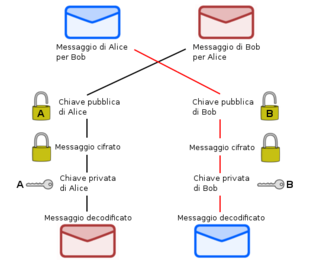
\includegraphics[width=3cm]{../assets/310px-Crittografia_asimmetrica_schema.png}
\caption{crittografia asimmetrica}
\end{figure}

\begin{enumerate}
\def\labelenumi{\arabic{enumi}.}
\tightlist
\item
  Bob cripta il messaggio con la chiave pubblica di Alice;
\item
  Alice decripta il messaggio di Bob con la sua chiave Privata.
\end{enumerate}

Ovviamente, nel caso in cui sia Alice a voler inviare un messaggio a
Bob, ella eseguirà gli stessi passaggi di Bob, il quale invece farà come
aveva fatto Alice.

\hypertarget{canali-pubblici-con-messaggi-firmati}{%
\subsubsection{Canali pubblici con messaggi
firmati}\label{canali-pubblici-con-messaggi-firmati}}

Alice ha bisogno di comunicare ad un gruppo di persone un qualche
messaggio e decide di farlo apponendo una firma ``digitale'' al suo
messaggio cosicchè tutto i destinatari possano controllare che nessun
altro ha cambiato il contenuto di quello che Alice voleva comunicare e
che è stata proprio lei, e non un altro, a scrivere il messaggio.

\begin{figure}
\centering
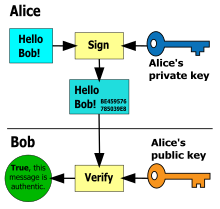
\includegraphics[width=3cm]{../assets/220px-Illustration_of_digital_signature.svg.png}
\caption{firma digitale asimmetrica}
\end{figure}

\begin{enumerate}
\def\labelenumi{\arabic{enumi}.}
\tightlist
\item
  Alice crea una cosidetta impronta del suo messaggio, applicando una
  funzione di \emph{hash} ad esso e producendo una stringa
\item
  Alice cifra il risultato dell'hash con la sua chiave privata, il
  risultato dell codifica è la firma digitale di Alice per quel
  messaggio
\item
  Alice allega la firma digitale al messaggio in chiaro e invia tutto ai
  suoi destinatari
\item
  Bob e chiunque altro riceva il messaggio, controlla che l'hash (lo
  stesso algoritmo di Alice) del messaggio in chiaro corrisponda con il
  risultato della decifratura della firma; quest'ultima fatta con la
  chiave pubblica di Alice.
\end{enumerate}

\hypertarget{monitoraggio-della-rete}{%
\subsection{Monitoraggio della rete}\label{monitoraggio-della-rete}}

L'ultimo componente - ma non per questo meno importante - del nostro
sistema, è il \emph{monitor} di rete. Esso si occupa di trascrivere
(indifferentemente in un file oppure su console) il log di sistema. Ogni
operazione invocata nella rete deve, subito prima o subito dopo, inviare
un messaggio di log al \emph{monitor}.

La sua interfaccia dovrebbe apparire simile alla seguente:

\begin{verbatim}
interface IMonitor {
    RequestResponse:
        log( string )( void )
}
\end{verbatim}

Dove, per semplicità, il tipo della richiesta dell'operazioe
\texttt{log} è una semplice stringa. L'uso di una operazione di tipo
\texttt{RequestResponse}, che implementa una comunicazione bloccante
vuole forzare il ``chiamante'' di questa operazione ad attendere finchè
il \emph{monitor} non ha ultimato la scrittura sulla coda dei
\emph{logs}. L'esempio è a titolo puramente esemplificativo e non
costituisce alcun obbligo nella scelta della soluzione pià appropriata
per questo componente.

\hypertarget{specifiche-per-la-consegna}{%
\section{Specifiche per la consegna}\label{specifiche-per-la-consegna}}

Globalmente, vengono consegnati due prodotti: la documentazione e
l'implementazione (il codice sorgente) del progetto. La valutazione
finale avviene mediante una esame orale, nella quale vengono discusse le
strategie con la quale i prodotti consegnati sono stati generati. Le
domande saranno rivolte a tutti i partecipanti al gruppo, i quali
potranno scegliere l'esposizione organizzata dei contenuti.

\begin{itemize}
\tightlist
\item
  non si accettano richieste di eccezioni sui progetti con motivazioni
  legate a esigenze di laurearsi
\item
  chi copia o fa copiare invalida il progetto - il codice viene
  controllato con un programma per il rilevamento di plagio - si rimanda
  alla pagina del tutor per maggiori informazioni sul
  \href{https://spz.netlify.app/teaching/2020/02/24/operative-system-laboratory-computer-science-management}{codice
  d'onore} del laboratorio.
\end{itemize}

\hypertarget{la-documentazione}{%
\subsection{La documentazione}\label{la-documentazione}}

È possibile scrivere la documentazione nel formato preferito,
l'importante è che il PDF generato rispetti la struttura del modello
(più avanti). La documentazione ha lunghezza di \textbf{almeno} quattro
o cinque pagine (quindi da 8 a 10 facciate), è scritto con font di
grandezza \emph{12pt} e viene consegnato in formato PDF. Il limite è un
\emph{lower bound}; non esiste un \emph{upper bound} per la lunghezza
del report che può quindi essere di un numero arbitrario di pagine.

Di seguito viene riportato un esempio di documentazione con le
principali caratteristiche da inserire.

\hypertarget{lintestazione-della-documentazione}{%
\paragraph{L'intestazione della
Documentazione}\label{lintestazione-della-documentazione}}

\begin{itemize}
\tightlist
\item
  Laboratorio Sistemi Operativi A.A. 2019-2020
\item
  Nome del Gruppo
\item
  Indirizzo mail del referente: nome.cognome@studio.unibo.it
\item
  Componenti:

  \begin{itemize}
  \tightlist
  \item
    Cognome, Nome, Matricola
  \item
    \ldots{}
  \end{itemize}
\end{itemize}

\hypertarget{il-corpo-della-documentazione}{%
\paragraph{Il corpo della
Documentazione}\label{il-corpo-della-documentazione}}

\begin{enumerate}
\def\labelenumi{\arabic{enumi}.}
\tightlist
\item
  Descrizione generale del progetto

  \begin{enumerate}
  \def\labelenumii{\arabic{enumii}.}
  \tightlist
  \item
    Componenti del progetto
  \item
    Funzionalità implementate
  \item
    Contenuto della documentazione
  \end{enumerate}
\item
  Istruzioni per la demo - le istruzioni per eseguire una demo.
\item
  Discussione sulle strategie di implementazione:

  \begin{enumerate}
  \def\labelenumii{\arabic{enumii}.}
  \tightlist
  \item
    Struttura del progetto - come è stato diviso il progetto tra i
    componenti del grupppo. Quali sono i problemi principali riscontrati
    nell'implementazione? Quali sono le alternative considerate? Perché
    sono state adottate alcune soluzinoi piuttosto di altre?
  \item
    Sezione di descrizione della - ad esempio, abbiamo implementato
    l'operazione \texttt{foo} perché abbiamo bisogno di \ldots{} Il
    codice di esempio (riporto il codice) mostra il problema appena
    descritto \ldots{} risolto con \ldots{}
  \end{enumerate}
\end{enumerate}

In ogni caso motivare le proprie scelte giustificando le proprie azioni.

\hypertarget{griglia-di-valutazione-per-la-documentazione}{%
\subsubsection{Griglia di Valutazione per la
documentazione}\label{griglia-di-valutazione-per-la-documentazione}}

La valutazione della documentazione verte sull'analisi dello scritto e
sulla sua capacità di esprimere con chiarezza i concetti descritti,
soprattutto \textbf{grazie all'uso di esempi}.

In particolare la griglia di valutazione usata è la seguente:

\begin{longtable}[]{@{}ll@{}}
\toprule
\begin{minipage}[b]{0.47\columnwidth}\raggedright
Criterio\strut
\end{minipage} & \begin{minipage}[b]{0.47\columnwidth}\raggedright
Descrizione\strut
\end{minipage}\tabularnewline
\midrule
\endhead
\begin{minipage}[t]{0.47\columnwidth}\raggedright
\textbf{Qualità dell'informazione}\strut
\end{minipage} & \begin{minipage}[t]{0.47\columnwidth}\raggedright
Riconoscimento dei problemi (di concorrenza) e loro descrizione\strut
\end{minipage}\tabularnewline
\begin{minipage}[t]{0.47\columnwidth}\raggedright
\textbf{Uso degli esempi}\strut
\end{minipage} & \begin{minipage}[t]{0.47\columnwidth}\raggedright
Presenza di almeno un esempio in tutte le scelte implementative\strut
\end{minipage}\tabularnewline
\begin{minipage}[t]{0.47\columnwidth}\raggedright
\textbf{Analisi delle scelte implementative}\strut
\end{minipage} & \begin{minipage}[t]{0.47\columnwidth}\raggedright
Descrizione della propria scelta implementativa e presenza di proposte
di alternative valide\strut
\end{minipage}\tabularnewline
\bottomrule
\end{longtable}

\hypertarget{limplementazione-del-progetto}{%
\subsection{L'implementazione del
progetto}\label{limplementazione-del-progetto}}

Il progetto viene sviluppato utilizzando il linguaggio Jolie. Non ci
sono requisiti riguardo ai protocolli \emph{protocolli} e i \emph{media}
utilizzati per realizzare la comunicazione tra i componenti del sistema.

La gestione del progetto avviene col supporto del sistema \texttt{git},
a
\href{https://education.github.com/git-cheat-sheet-education.pdf}{questa
pagina} è possibile trovare una lista di comandi utili per imparare ad
usare questo strumento di scrittura collaborativa.

Il codice del progetto è contenuto in uno spazio in cloud del servizio
online \href{http://gitlab.com}{GitLab} e gestito seguendo la procedura
descritta di seguito.

\textbf{N.B. Le istruzioni che seguono devono essere completate entro e
non oltre la scadenza di presentazione dei gruppi.}

\begin{enumerate}
\def\labelenumi{\arabic{enumi}.}
\tightlist
\item
  Ogni membro del gruppo \href{https://gitlab.com/users/sign_in}{crea un
  account su GitLab o accede con le proprie credenziali}
\item
  Il \textbf{referente del gruppo} crea un nuovo progetto cliccando sul
  bottone \textbf{+} in alto a destra nella schermata principale di
  GitLab, inserendo \texttt{LabSO\_NomeGruppo} come nome del progetto e
  cliccando su \textbf{New Project}

  \begin{itemize}
  \tightlist
  \item
    una volta che il progetto è stato creato, il referente aggiunge ogni
    membro del gruppo con \texttt{role\ permission} \(>\)
    \texttt{Developer} andando su \texttt{Settings} \(>\)
    \texttt{Members} nel menù a sinistra, cercandoli in base allo
    username con il quale questi si sono registrati su GitLab;
  \item
    il referente aggiunge l'utente \texttt{stefanopiozingaro} con
    \texttt{role\ permission} \(>\) \texttt{Reporter}.
  \end{itemize}
\end{enumerate}

\hypertarget{la-consegna-dellimplementazione}{%
\subsection{La consegna
dell'implementazione}\label{la-consegna-dellimplementazione}}

Al momento della consegna, il repository dovrà contenere i sorgenti del
progetto e la relazione, nominata \texttt{REPORT\_LSO.pdf}.

Per effettuare la consegna:

\begin{enumerate}
\def\labelenumi{\arabic{enumi}.}
\tightlist
\item
  Nella pagina del progetto, cliccare sulla voce del menù
  \texttt{Repository} \(>\) \texttt{Tags} \(>\) \texttt{New\ Tag}
\item
  Digitare come \texttt{Tag\ Name} il nome \textbf{Consegna}
\item
  Cliccare su \texttt{Create\ Tag} per eseguire la creazione del
  \texttt{Tag} di consegna
\end{enumerate}

Una volta creato il Tag, inviare una email di notifica di consegna con
soggetto \textbf{CONSEGNA LSO - NOME GRUPPO} a
stefanopio.zingaro@unibo.it.

\hypertarget{griglia-di-valutazione-per-limplementazione}{%
\subsubsection{Griglia di Valutazione per
l'implementazione}\label{griglia-di-valutazione-per-limplementazione}}

La valutazione dell'implementazione del sistema si basa sull'analisi del
codice Jolie, sull'uso dei costrutti del linguaggio per la creazione di
soluzioni efficienti, sulla tolleranza ai guasti del sistema
implementato e sulla gestione delle eccezioni.

In particolare la griglia di valutazione usata è la seguente:

\begin{longtable}[]{@{}ll@{}}
\toprule
\begin{minipage}[b]{0.47\columnwidth}\raggedright
Criterio\strut
\end{minipage} & \begin{minipage}[b]{0.47\columnwidth}\raggedright
Descrizione\strut
\end{minipage}\tabularnewline
\midrule
\endhead
\begin{minipage}[t]{0.47\columnwidth}\raggedright
\textbf{Uso dei costrutti di Jolie}\strut
\end{minipage} & \begin{minipage}[t]{0.47\columnwidth}\raggedright
Corretto utilizzo dei costrutti per la gestione della concorrenza, uso
corretto di \texttt{execution(...)}\strut
\end{minipage}\tabularnewline
\begin{minipage}[t]{0.47\columnwidth}\raggedright
\textbf{Distribuzione del carico di lavoro nel gruppo}\strut
\end{minipage} & \begin{minipage}[t]{0.47\columnwidth}\raggedright
Omogeneità nella ripartizione dei compiti nel gruppo, ogni membro
partecipa egualmente allo sviluppo indicando il singolo contributo,
assenza di dissimmetria di informazione.\strut
\end{minipage}\tabularnewline
\begin{minipage}[t]{0.47\columnwidth}\raggedright
\textbf{Grado di partecipazione alla comunità}\strut
\end{minipage} & \begin{minipage}[t]{0.47\columnwidth}\raggedright
Presenza di domande e risposte significative sui canali di comunicazione
offerti dal corso, richieste di ricevimento e delucidazioni, bug fixing
del materiale messo a disposizione del docente e dalla comunità
\emph{open source} di Jolie\strut
\end{minipage}\tabularnewline
\bottomrule
\end{longtable}

\hypertarget{la-dimostrazione-demo}{%
\subsection{La dimostrazione (demo)}\label{la-dimostrazione-demo}}

Insieme alla documentazione ed al codice sorgente, dovrà essere
preparato uno script che permette di automatizzare i test. Almeno nella
fase iniziale della prova orale, può essere utile preparare del
materiale da correlare allo script (ad esempio \emph{screenshot}), che
permetteranno di velocizzare le operazioni di controllo del codice. Tale
suite di test \emph{può} essere intergrata nel codice sorgente (è
tuttavia opzionale).

\end{document}
